\section{Similar Face Recognition Using the IE-CNN Model}

\begin{center}
    \author{
    An-Ping Song,
    Qian Hu,
    Xue-Hai Ding,
    Xin-Yi Di,
    Zi-Heng Song
    }
\end{center}

\begin{center}
    \emph{DIGITAL OBJECT IDENTIFIER}
\end{center}

\subsection{INTRODUCTION}
Currently there are few datasets that provide a set of images with faces of 
similar people, moreover there are few methods tested to be able to verify 
the level of similarity. Two types of work are carried out in the following paper. 
The first is based on proposing a procedure for creating a large dataset of 
similar faces that requires a small amount of man-force to label the content. 
In the second work, instead, an IE-CNN model is built which has the task 
of improving the internal and external features of the face, increasing the 
precision of face matching.

\subsection{RELATED WORK}
Unlike objects that may have a similar shape or color, the human face may 
have similar external (located at head, chin and ears) or internal (eyes, nose 
and mouth) structural features. However, many recognition algorithms tend 
to discard external features and only work with internal ones. To understand 
the importance of using both categories of features, just look at the image \ref{fig:features} 
where there are similar faces (internal features) but different physical structures 
of the skull (external features), or the opposite. The proposed model 
(\emph{IE-CNN}) deals with improving facial features using a CNN network.
\begin{figure}[h!]
    \centering
    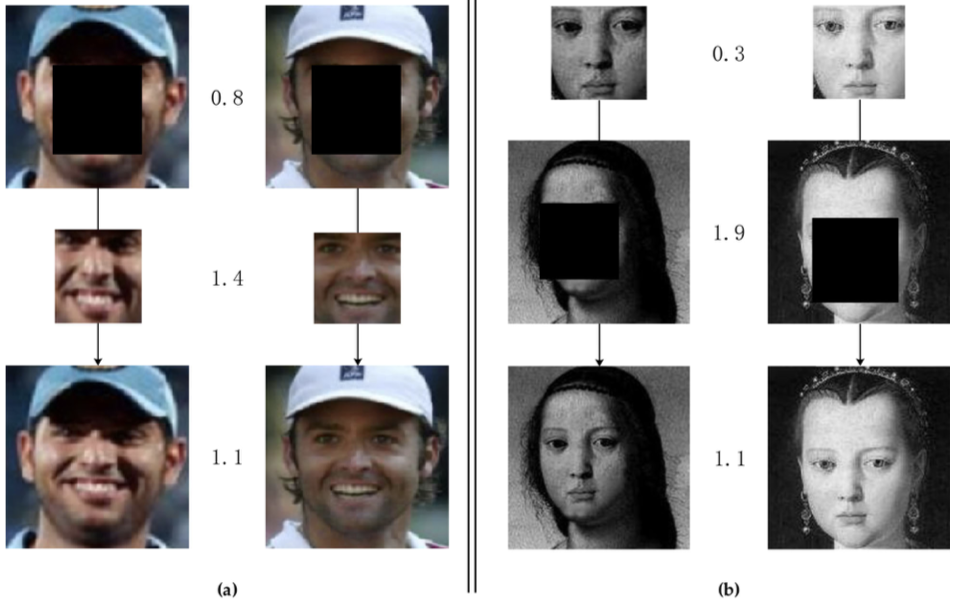
\includegraphics[width = 0.8\linewidth]{images/paper9/importance.png}
    \centering
    \caption{(a) Shows the importance of internal features and (b) shows the importance of external features. The values are the cosine distances.}
    \label{fig:features}
\end{figure}

\subsection{DATASET COLLECTION}
The creation of the proposed similar-face dataset (SFD) consists of several steps.
\begin{enumerate}
    \item \emph{Collecting The Suitable Data Source}: the dataset used to collect the faces are LFW and CASIA-WebFace. The first contains a set of images of faces collected from the network, while the second has faces appropriately selected and labeled.
    \item \emph{Determining the Similarity Between Two Faces Images}: to measure the similarity of two faces, the calculation of the distance $L2$ on image vectors is used.
    \item \emph{Generating the Similar FaceDataset (SFD)}:if vectors with a short distance are found, then this distance will be stored. Based on the distance value, this can be associated with a grade type. The images belonging to the same grade, and therefore with the same distance, will be grouped.
\end{enumerate}